\documentclass[11pt]{article}
\usepackage[margin=2cm]{geometry}
\usepackage{amsmath,amssymb}
\usepackage{graphicx}
\usepackage{booktabs}
\usepackage[hidelinks]{hyperref}
\hypersetup{pdfauthor={Feiyang Zhong and Haoyang Feng},
            pdftitle={Snow Divides: do snow seasons draw the climate boundaries of the Tibetan Plateau?}}
\usepackage[font=small,labelfont=bf]{caption}
\setlength{\parskip}{0.45em}
\setlength{\parindent}{0pt}
\graphicspath{{figures/}}

\begin{document}

\begin{center}
  {\small CS-521 / CS-321 / Math-462, Fall 2026 \hfill Homework 1, Part II (Experiment)}\\[0.8em]
  {\Large\bfseries Snow Divides: do snow seasons draw the climate\\[0.2em] boundaries of the Tibetan Plateau?}\\[0.8em]
  Feiyang Zhong \quad and \quad Haoyang Feng\\[0.3em]
  {\small Code: \url{https://github.com/Wade-Zhong05/snow-divides}}
\end{center}

\section*{Question}

The Tibetan Plateau lies between two climates: the mid-latitude \emph{westerlies} in the
northwest and the Indian \emph{monsoon} in the southeast, with a transition zone between
them. The divide matters because glaciers behave differently on each side: they are
stable or advancing in the northwest and retreat fastest in southeast Tibet
\cite{yao2012}. Snow records when precipitation falls and how cold it is, so the
\emph{shape} of a place's snow season should carry the same signature.

\textbf{Research question.} \emph{From snow alone, does a kNN graph of snow-season shapes
recover the climate regions of the plateau? Are the boundaries between them sharp divides
or broad transition zones that shift from year to year?} We test three hypotheses:
\textbf{H1} the graph's regions are spatially coherent, match the westerly / transition /
monsoon pattern and are not explained by elevation; \textbf{H2} the boundaries are broad,
shifting belts rather than lines; \textbf{H3} part of the structure comes from
non-climate factors (elevation, glacier ice, satellite sensor changes).

%=======================================================================
\section*{E-1 \quad Data and feature extraction}

\textbf{Data.} \emph{Long-term series of daily snow depth dataset in China}
\cite{che_data,che2008,dai2015,dai2017}, from the National Tibetan Plateau Data Center
(TPDC): daily snow depth (cm) on a $0.25^\circ$ grid, retrieved from satellite
passive-microwave radiometers. We use the plateau window $26$--$40^\circ$N,
$73$--$105^\circ$E ($57\times129=7{,}353$ cells) and 14 \emph{snow years} 2000/01--2013/14,
each running 1~Aug--31~Jul and built from two consecutive calendar years. Two further
TPDC datasets are used only to \emph{interpret} the results, never as features: a DEM
(band 41 of the snowmelt-onset product \cite{xiong_data,xiong2017,xiong2019}) and the 82
glaciers of Table~S4 of Yao et al.\ \cite{yao_data,yao2012}, with coordinates, region
(I--VII) and 1970s--2000s length change.

\textbf{Datum and attributes.} A datum $x_j$ is one grid cell; its attribute is a
numerical array of $14\times365$ daily depths. We keep cells with at least 60 snow days
per year on average (depth $>0.5$\,cm): \textbf{3,238 cells}.

\textbf{Feature-equivalent data are contracted (Part I, 1.1.3).} 101 pairs of horizontally
adjacent cells have \emph{identical} depth on all 5,110 days. They lie in five columns
spaced $6.25^\circ$ apart ($78.75$, $85.25$, $91.5$, $97.75$, $104.0^\circ$E), which is
consistent with regridding from a source grid slightly coarser than $0.25^\circ$ in
longitude. Each pair is one feature-equivalence class and becomes one vertex:
\textbf{$n = 3{,}137$ vertices}.

\textbf{Feature: multi-scale temporal HOG} (our answer to optional question 1-b). A cell's
depth curve $s(t)$ is treated as a shape in the (day, depth) plane (Fig.~\ref{fig:e1}).
For each time lag $L \in \{1, 7, 15, 31, 61\}$ days:
\begin{itemize}\setlength\itemsep{0.1em}
  \item the rate of change over $L$ days is
        $r_L(t) = \big(s(t+\lceil L/2\rceil) - s(t-\lfloor L/2\rfloor)\big)/L$ (cm/day);
  \item its \emph{orientation} is $\theta = \arctan(r_L/c)$ with $c = 0.3$\,cm/day; six
        signed bins over $(-90^\circ, 90^\circ)$ give \emph{fast melt, melt, slow melt, slow
        accumulation, accumulation, fast accumulation};
  \item each day votes $|r_L(t)|$ into its bin (split linearly between the two nearest
        bins); votes are summed over \emph{half-month cells} (24 per year);
  \item blocks of two consecutive cells are L2-Hys normalised (clip 0.2,
        $\varepsilon = 1$\,cm) \cite{dalal2005}, averaged over the 14 years and normalised
        to sum to 1.
\end{itemize}
The five lag blocks are concatenated with equal weight:
$d = 5 \times 24 \times 2 \times 6 = 1440$. A difference over $L$ days averages out
changes shorter than $L$ days, so the five lags see the snow season at five time scales,
from single snowfalls to the seasonal build-up and melt (a scale-space description
\cite{lindeberg1994}). As in HW 1.1.5, gradients ignore a constant offset, so a permanent
signal (e.g.\ glacier ice) contributes nothing by itself. Block normalisation removes the
\emph{amount} of snow, so the feature describes \emph{when} and \emph{how fast} snow comes
and goes.

\begin{figure}[h]
  \centering
  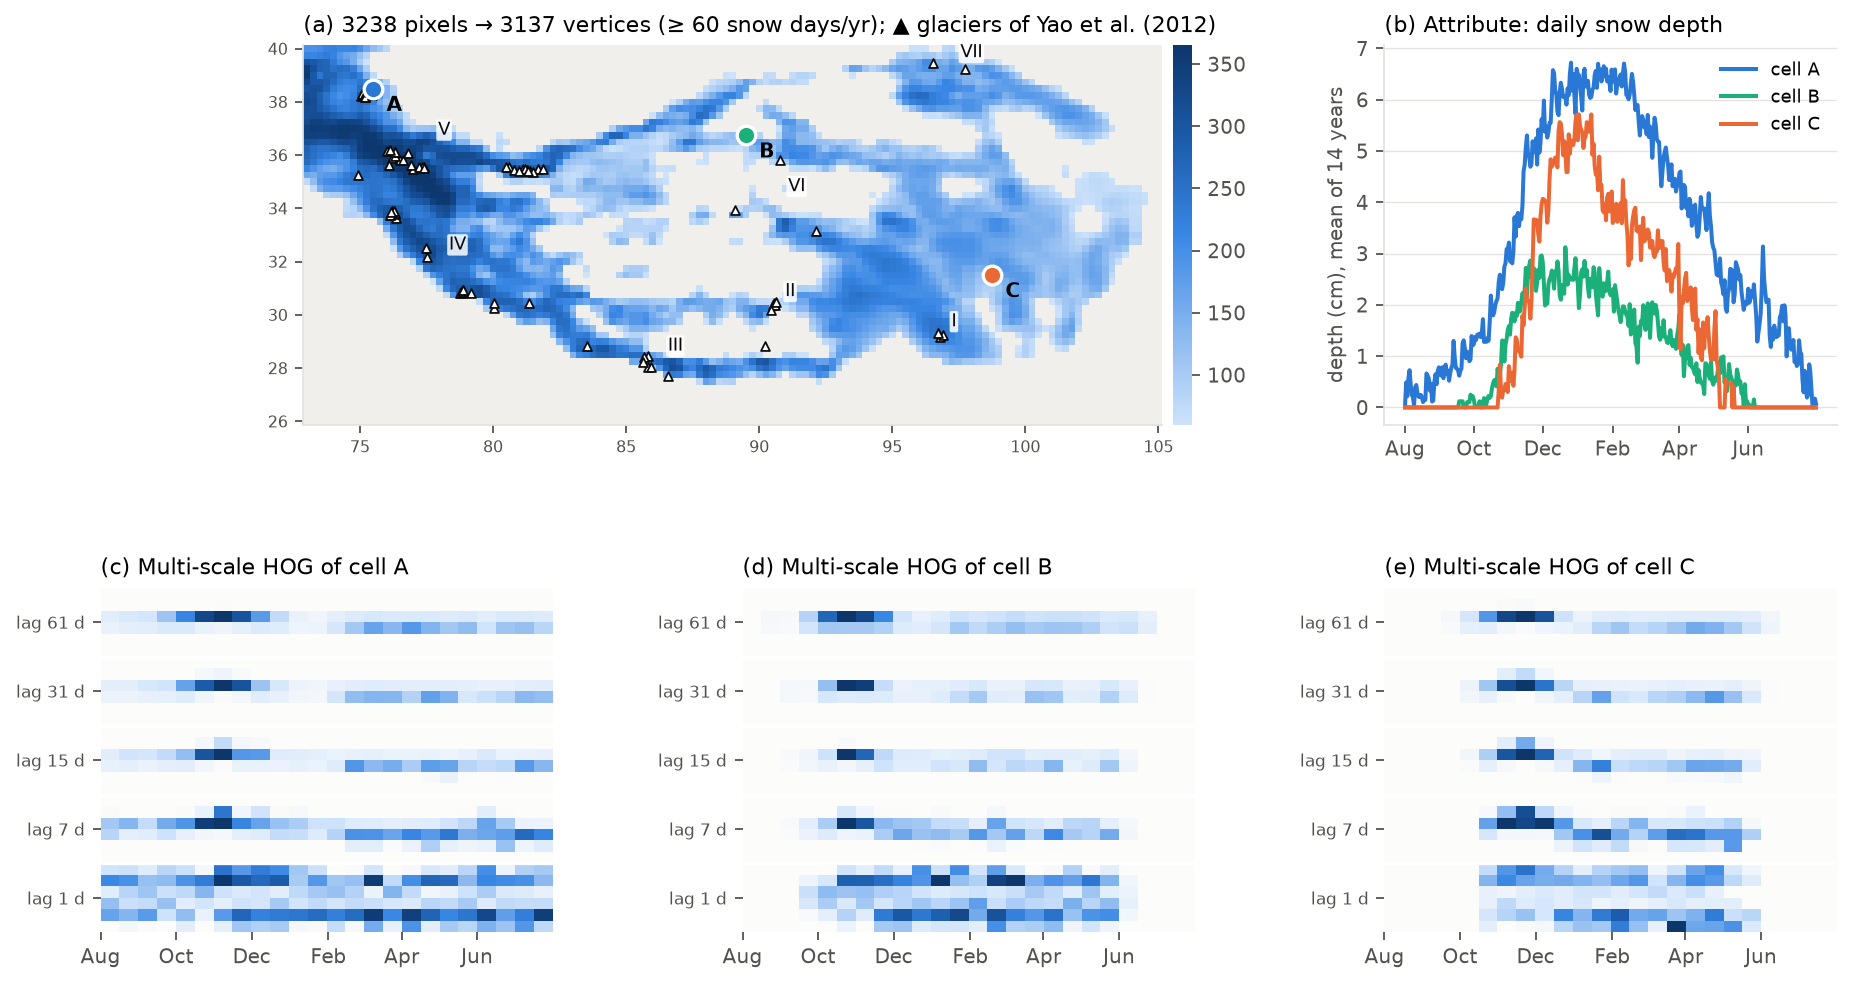
\includegraphics[width=\textwidth]{e1_data_features.png}
  \caption{(a) The 3,238 cells and their mean number of snow days; triangles are the
  glaciers of Yao et al.\ (2012), labelled by region. (b) Mean snow year of three
  representative cells (the medoids of the three regions found in E-6). (c--e) Their
  multi-scale HOG, drawn from the 14-year mean curve for display (the feature itself
  averages the HOG of each year): one block per lag, each scaled to its own maximum; in
  each block the six rows are the slope bins, from fast melt (bottom) to fast
  accumulation (top). The 1-day block of every cell is
  spread over fast melt and fast accumulation (day-to-day flicker); the 15--61-day blocks
  show the season: slow accumulation in October--December, slow melt from February.}
  \label{fig:e1}
\end{figure}

\textbf{The feature is a hyperparameter: we compared 13 candidates.} Every candidate went
through the same pipeline (E-2 to E-6, $k=21$, $K=3$) on the same vertices. No ground
truth exists, so each was scored on independent checks (Table~\ref{tab:features},
Fig.~\ref{fig:lags}). \emph{Glacier purity}: share of the 74 glaciers of Yao et al.\ that
lie in their group's region (groups V+IV, II+VI+VII, I; region III is mixed and left
out). \emph{Contiguity}: share of map-neighbour pairs in the same region; chance is
about 0.35, and the features contain no location. \emph{Climate}:
$|r(q_2, \text{longitude})|$ among cells at 4,400--5,000\,m. \emph{Elev.\ $\eta^2$}:
share of elevation variance explained by the regions (lower is better). \emph{Split}:
two graphs built from disjoint halves of the years (7/7, five random splits), compared by
the adjusted Rand index (ARI) of their partitions and by the share of 21 nearest
neighbours they have in common. \emph{Era}: the same neighbour overlap between
2000/01--2007/08 and 2008/09--2013/14, which straddle a sensor change.

\begin{table}[h]
\centering\small
\resizebox{\textwidth}{!}{%
\begin{tabular}{llrcccccc}
\toprule
Family & Feature & $d$ & glacier purity & contiguity & climate & elev.\ $\eta^2$ & split ARI & split / era kNN \\
\midrule
no gradient & raw depth per half-month & 24 & 0.99$^\dagger$ & 0.85 & 0.78 & 0.23 & $0.72\pm0.07$ & 0.37 / 0.30 \\
            & share of snow days per half-month & 24 & 0.93 & 0.76 & 0.55 & 0.05 & $0.74\pm0.05$ & 0.28 / 0.17 \\
day-count gradient & first prototype: day counts + snow-day share & 240 & 0.91$^\dagger$ & 0.87 & 0.67 & 0.15 & $0.73\pm0.02$ & 0.22 / 0.16 \\
(1 vote per day) & day counts only & 240 & 0.91$^\dagger$ & 0.80 & 0.58 & 0.10 & $0.24\pm0.06$ & 0.15 / 0.11 \\
HOG, one lag & 1 day & 288 & 0.95$^\dagger$ & 0.84 & 0.75 & 0.13 & $0.73\pm0.05$ & 0.28 / 0.20 \\
(votes $=|r_L|$) & $\approx$2 days, smoothed (earlier draft) & 288 & 0.99 & 0.87 & 0.74 & 0.13 & $0.42\pm0.13$ & 0.39 / 0.31 \\
            & 7 days & 288 & 0.97 & 0.87 & 0.77 & 0.12 & $0.55\pm0.16$ & 0.42 / 0.32 \\
            & 31 days & 288 & 0.99 & 0.88 & 0.82 & 0.10 & $0.72\pm0.07$ & 0.48 / 0.39 \\
HOG, multi-scale & 7, 15, 31, 61 days & 1152 & 0.99 & 0.88 & \textbf{0.83} & 0.10 & $0.76\pm0.06$ & \textbf{0.53} / \textbf{0.43} \\
            & \textbf{1, 7, 15, 31, 61 days (chosen)} & 1440 & \textbf{0.99} & \textbf{0.88} & 0.82 & \textbf{0.09} & $\mathbf{0.78\pm0.04}$ & \textbf{0.53} / 0.42 \\
signal analysis & Haar wavelet energy, 2--64-day scales & 144 & 0.72 & 0.87 & 0.77 & 0.04 & $0.42\pm0.08$ & 0.46 / 0.39 \\
            & Fourier harmonics 1--6 of the annual cycle & 12 & 0.92$^\dagger$ & 0.88 & 0.72 & 0.26 & $0.56\pm0.03$ & 0.31 / 0.26 \\
            & phenology (onset, melt-out, duration, \dots) & 8 & 0.99$^\dagger$ & 0.85 & 0.65 & 0.16 & $0.39\pm0.17$ & 0.20 / 0.14 \\
\bottomrule
\end{tabular}}
\caption{E-1: feature comparison (same vertices, same graph pipeline). $^\dagger$The
three glacier groups do not fall into three different regions (for example, southeast
Tibet is grouped with the west), even when the purity is high.}
\label{tab:features}
\end{table}

\begin{figure}[h]
  \centering
  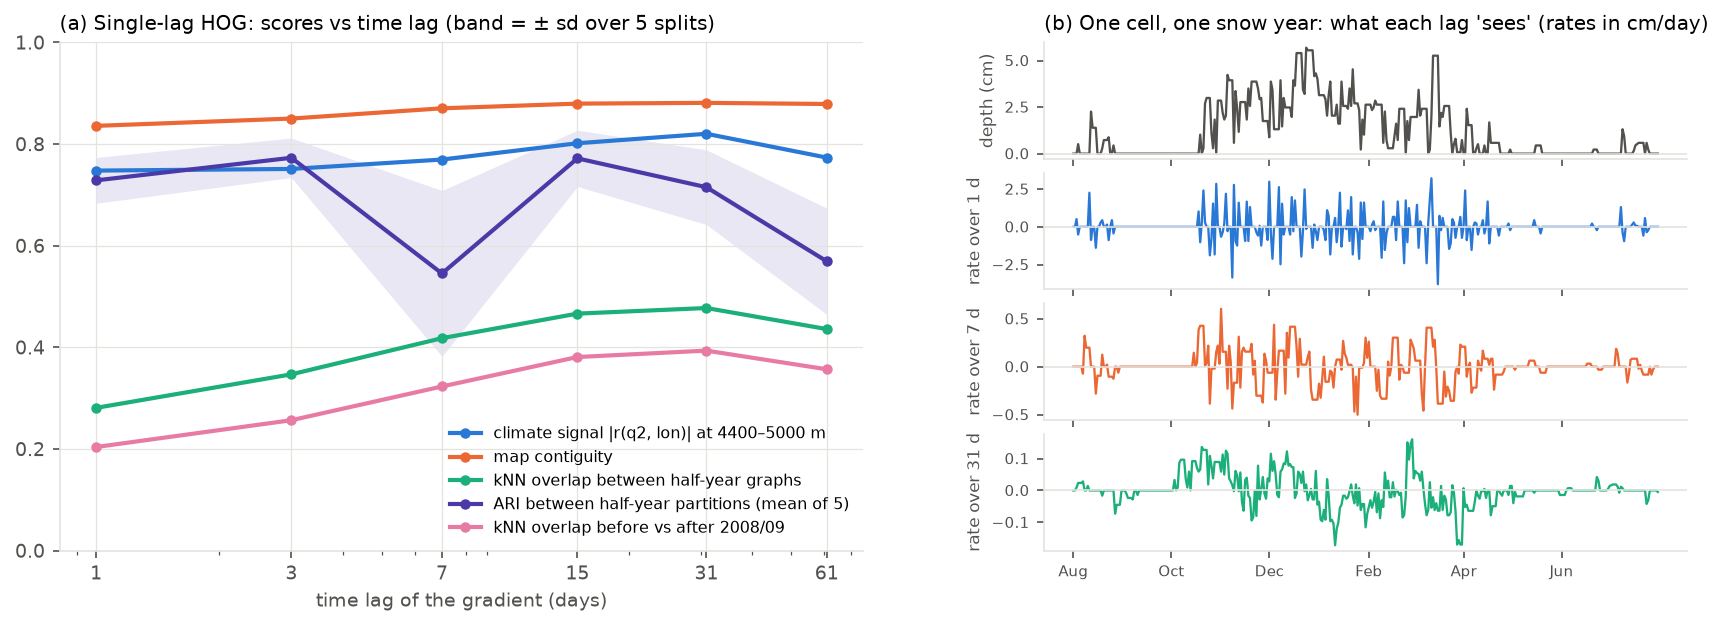
\includegraphics[width=\textwidth]{compare_lags.png}
  \caption{(a) Single-lag HOG: scores versus the time lag of the gradient. (b) One cell in
  one snow year: its depth, and the rate of change over 1, 7 and 31 days.}
  \label{fig:lags}
\end{figure}

\textbf{What the comparison shows.} Daily depth from passive microwave flickers by
several centimetres from one day to the next (Fig.~\ref{fig:lags}b). A 1-day gradient
mostly sees this flicker, while differences over 2--8 weeks see the seasonal build-up and
melt. Scores rise with the lag up to about a month (Fig.~\ref{fig:lags}a). Combining
several lags is best or tied for best on every check except $\eta^2$, where only two
features that fail other checks score lower. Counting \emph{days} per gradient bin (our first
prototype) gives the flicker the same weight as real snowfall; without the snow-day share
it is the least stable feature. The raw depth curve and the Fourier harmonics keep the
\emph{amount} of snow and follow elevation ($\eta^2 = 0.23$, $0.26$). We therefore use
the multi-scale HOG with lags 1, 7, 15, 31 and 61 days. Keeping the 1-day block does not
hurt and slightly stabilises the partition ($0.78\pm0.04$ vs.\ $0.76\pm0.06$). The other
hyperparameters matter little for this feature. Monthly or weekly cells
($d = 720$, $2880$) give the same three regions for 99\% of the cells. A snow-day
threshold of 30 or 90 days (3,686 or 2,643 vertices) gives the same regions for 96\% and
97\% of the shared cells, with the three glacier groups separated in every case.

%=======================================================================
\section*{E-2 \quad Pairwise feature interaction matrix}

The features are probability distributions, so we use a stochastic measure, the
Hellinger distance
\[
  D_{ij} = \tfrac{1}{\sqrt2}\,\big\|\sqrt{f_i} - \sqrt{f_j}\big\|_2
         = \Big(1 - \textstyle\sum_m \sqrt{f_{im} f_{jm}}\Big)^{1/2},
\]
with the square root taken entrywise. It is a metric with values in $[0,1]$, it is
defined when some bins are zero, and the whole matrix is one matrix product. That speed
mattered: the comparison in E-1 built 13 graphs for each feature tested. As a check, the
square root of the Jensen--Shannon divergence, also a metric \cite{endres2003}, gives the
same 21 nearest neighbours in 96\% of cases. The $3137\times3137$ matrix has median 0.35
(5--95\%: 0.20--0.52), and its smallest off-diagonal entry is 0.002, so no exact
duplicates remain after contraction. Sorted by the regions found in E-6, it shows a clear
block structure (Fig.~\ref{fig:e2}).

\begin{figure}[h]
  \centering
  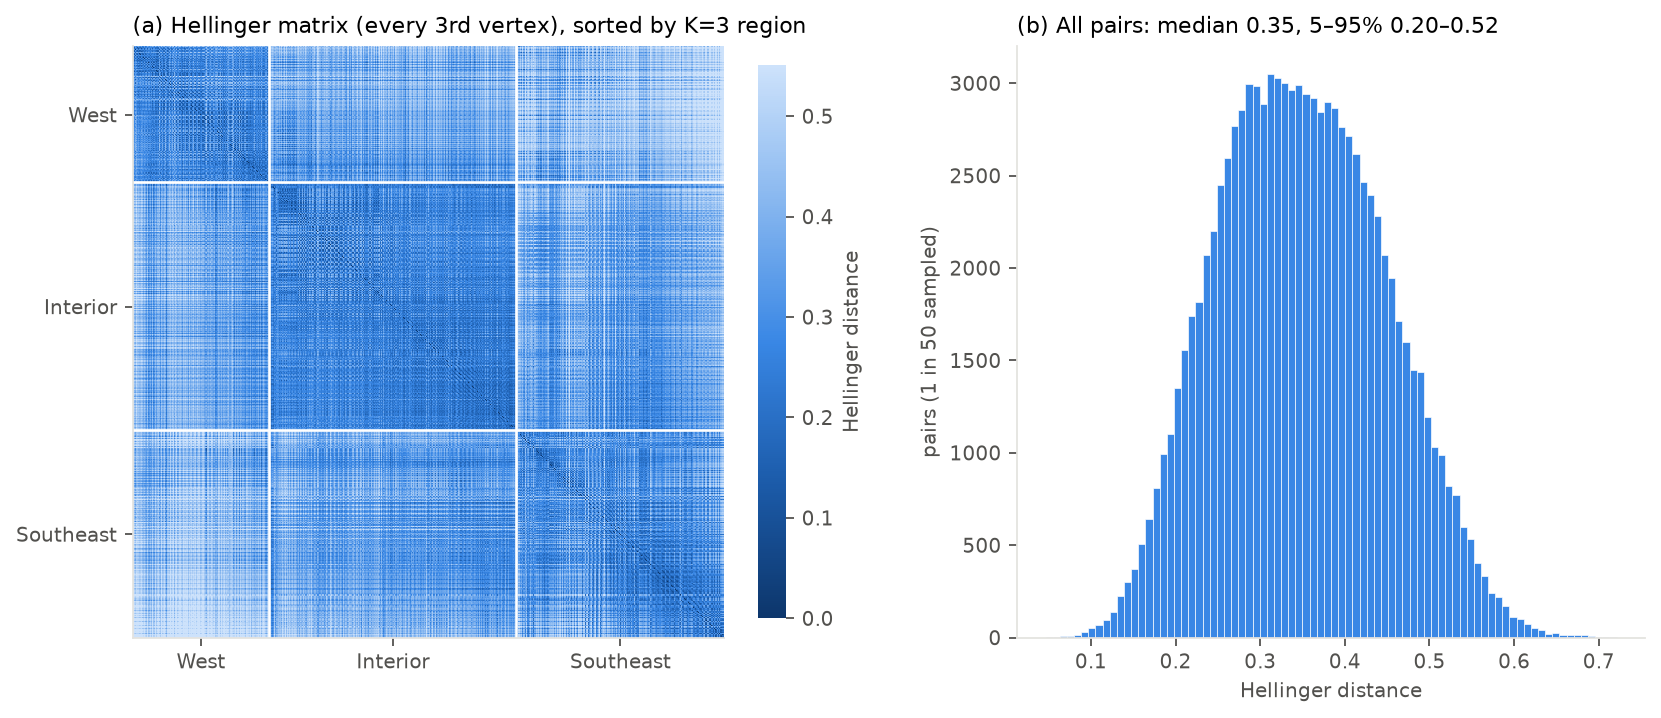
\includegraphics[width=0.95\textwidth]{e2_pairwise.png}
  \caption{(a) The Hellinger matrix (every third vertex), sorted by region and longitude;
  dark = similar. (b) Distribution of all pairwise distances.}
  \label{fig:e2}
\end{figure}

%=======================================================================
\section*{E-3 \quad kNN graphs and connected components}

\textbf{From $D$ to the adjacency matrix.}
\begin{enumerate}\setlength\itemsep{0.1em}
  \item For each row $i$ of $D$, set $D_{ii}=\infty$ and sort the row in ascending order
        (\texttt{argsort}). The first $k$ indices are the $k$ nearest neighbours of $i$.
        This gives a directed kNN matrix with exactly $k$ ones per row.
  \item Symmetrise by union, $A = A_{\rm dir} \lor A_{\rm dir}^{\top}$: $i$ and $j$ are
        adjacent if either one is among the other's $k$ nearest neighbours.
  \item Find the connected components by depth-first search.
\end{enumerate}
At $k=21$, 68\% of the directed relations are mutual, and the graph has 43,325 edges.

\textbf{Result} (Fig.~\ref{fig:e3}). We scanned the prescribed range $k\in[2^1, 2^6]$,
plus $k=1$. The graph has 857 components at $k=1$ and 23 at $k=2$, and it is
\textbf{connected from $k_c = 3$} up to 64. The 22 small components at $k=2$ have 3--21
cells each (115 vertices in total) and are scattered over the plateau. They are local
groups of unusual cells, not climate regions: \emph{the climate regions never appear as
separate components}. Even at $k=3$ they are joined through intermediate cells, a first
hint that the boundaries are gradual (H2).

\textbf{Choice of $k$.} We use $k = 21$ for E-4 to E-6. The choice is not critical: the
$K=3$ partition at $k = 16$, 32 and 64 agrees with the one at $k=21$ with ARI 0.96, 0.96
and 0.91 (0.84 at $k=8$).

\begin{figure}[h]
  \centering
  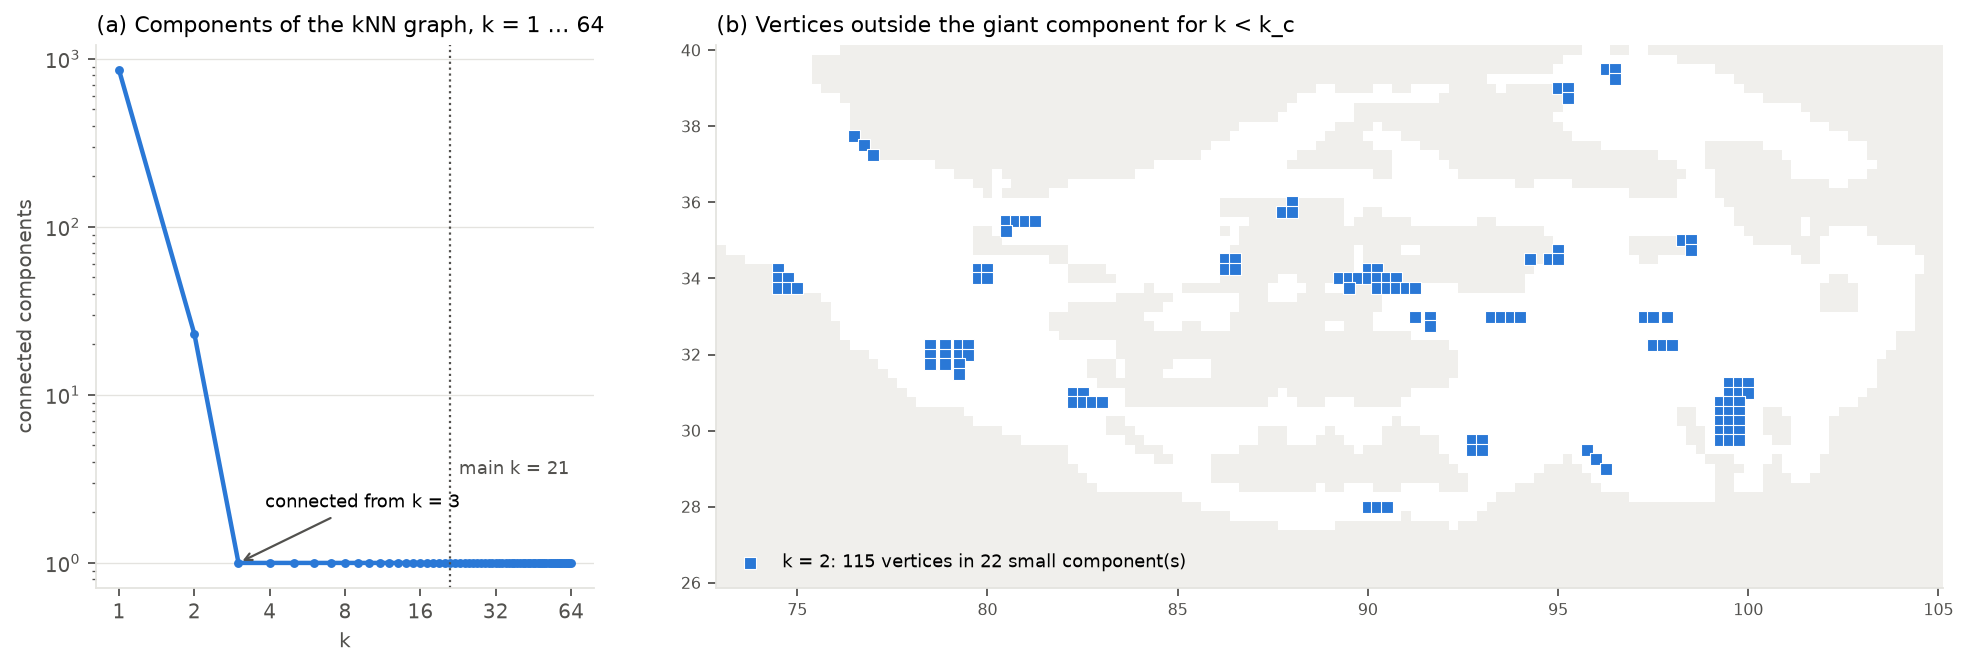
\includegraphics[width=\textwidth]{e3_components.png}
  \caption{(a) Number of connected components versus $k$, for $k = 1, \dots, 64$
  (log--log). (b) Vertices outside the giant component at $k=2$.}
  \label{fig:e3}
\end{figure}

%=======================================================================
\section*{E-4 \quad Combinatorial connectivity: degree and local clustering}

The graph at $k=21$ is a single component; Fig.~\ref{fig:e4} shows its distributions.

\textbf{Degree.} Every vertex has degree $\ge k = 21$ by construction. The degree equals
$k$ plus the number of vertices that choose $i$ without $i$ choosing them. The median is
26, the mean 27.6 and the maximum 73, and the distribution is right-skewed
(skewness 1.72). Its tail is a straight line on log-linear axes: an exponential fit of
$\log P(\deg \ge d)$ has $R^2 = 0.996$, against $0.978$ for a power law. So the degree
distribution is a \emph{shifted exponential (geometric-type)} distribution, not
scale-free. The high-degree vertices are ``hubs'' \cite{radovanovic2010}: typical snow
seasons that many cells pick as a neighbour. The tail is heavier than for kNN graphs of
uniformly random points with the same $n$ and $k$ (maximum degree 36--60 in 2 to 10
dimensions), which reflects the uneven density of snow-season shapes.

\textbf{Local clustering coefficient} $C_i = t_i / \binom{d_i}{2}$, with $t_i$ the number
of triangles through $i$, i.e.\ $(A^2\circ A)\,\mathbf{1}/2$ as in HW 1.2-h. The
distribution is unimodal and close to bell-shaped, with median 0.46 (5--95\%: 0.30--0.66).
This is far above a random graph of the same density ($\approx 0.009$): the kNN graph is
strongly clustered, like a mesh on a low-dimensional manifold. For comparison, kNN graphs
of uniformly random points give median clustering 0.59, 0.49, 0.42, 0.34 and 0.24 in 2, 3,
4, 6 and 10 dimensions. Our 0.46 lies between the 3-D and 4-D cases, which suggests (as a
rough heuristic) that the 1440-dimensional features lie near a manifold of only about
\emph{three to four} dimensions. On the map, clustering is lowest in the interior. It is
also lower on the west--interior and interior--southeast borders (medians 0.41 and 0.43)
than away from borders (0.48): the effect predicted for H2, though weak.

\begin{figure}[h]
  \centering
  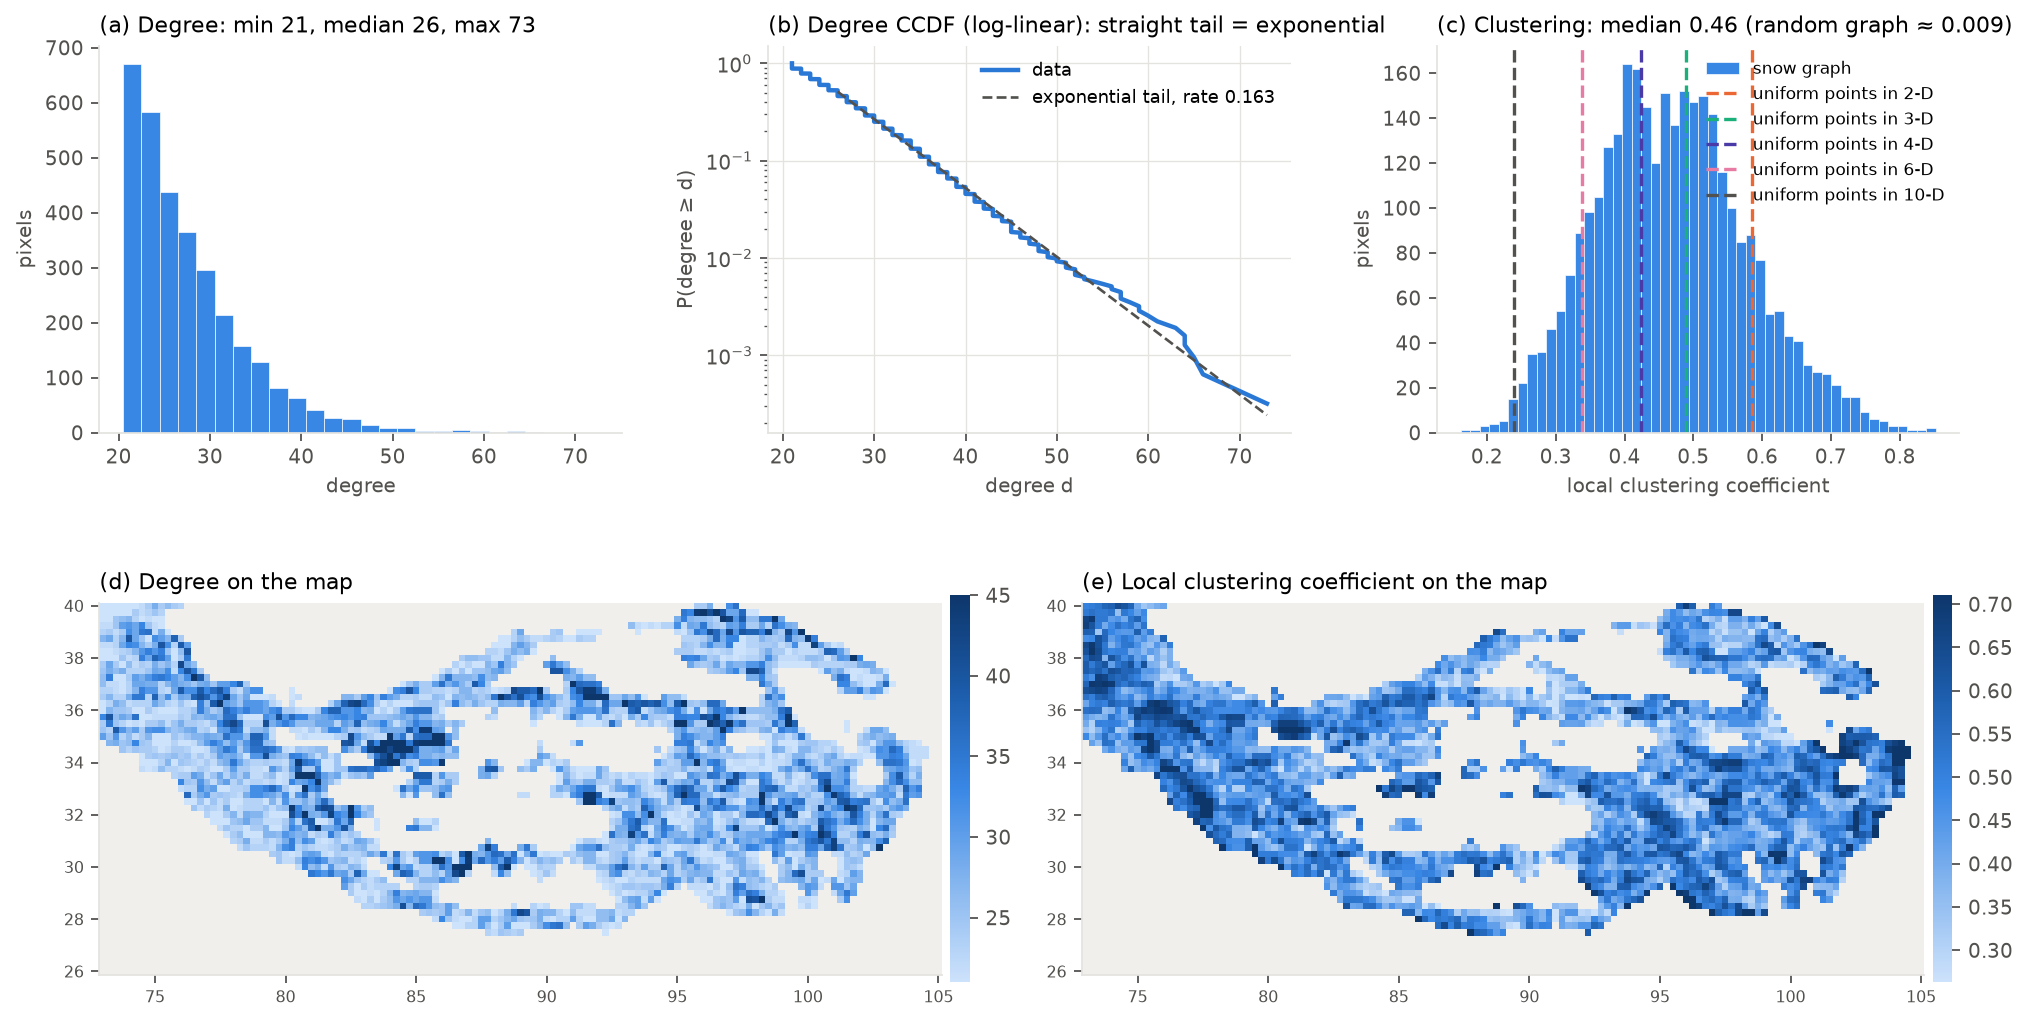
\includegraphics[width=\textwidth]{e4_degree_clustering.png}
  \caption{(a) Degree histogram. (b) Degree CCDF on log-linear axes with an exponential
  fit to the upper half. (c) Local clustering coefficient, with medians for kNN graphs of
  uniform random points in 2--10 dimensions (dashed). (d, e) Both quantities on the map.}
  \label{fig:e4}
\end{figure}

%=======================================================================
\section*{E-5 \quad Laplacian spectral analysis}

Edges carry self-tuning Gaussian weights $w_{ij} = \exp(-D_{ij}^2/(\sigma_i\sigma_j))$,
where $\sigma_i$ is the distance from $i$ to its 7th neighbour \cite{zelnik2004}. We form
$\hat L = I - D_w^{-1/2} W D_w^{-1/2}$.

\textbf{Fiedler value versus $k$.} The graph is connected for $k \ge k_c = 3$. As $k$
grows from 3 to 64, $\lambda_2(k)$ increases monotonically from 0.0017 to 0.0210 (0.0110 at
$k=21$). More neighbours add edges across the weakest cut, so the graph becomes better
connected algebraically (Fig.~\ref{fig:e5}b).

\textbf{Spectrum.} The 32 smallest eigenvalues at $k = 21$ (Fig.~\ref{fig:e5}a) rise
smoothly: $0$, $0.0110$, $0.0165$, $0.0223$, $0.0268$, $0.0347$, $0.0433$, \dots. We
measure separation by the smaller gap to an eigenvalue's two neighbours. The best
separated nonzero eigenvalue is $\lambda_6 = 0.0347$ (gaps 0.0079 below and 0.0086 above),
but only narrowly: $\lambda_2$ and $\lambda_3$ follow with 0.0055. The spectrum has no
strongly isolated eigenvalue, consistent with a continuum of snow seasons rather than
well-separated clusters. All 32 eigenvalues are simple (the closest pair differs by
0.0006).

\textbf{Nodal domains of $q_6$.} The nodal domains of $q_6$ are two connected subgraphs
of 1,606 ($q_6>0$) and 1,531 ($q_6<0$) vertices (Fig.~\ref{fig:e5}d). They do
\emph{not} follow the climate regions of E-6: each region is split roughly in half
(west 339/382, interior 729/587, southeast 538/562). They are only weakly related to snow
days, longitude or elevation ($|r| \le 0.24$). Within the west, they separate a stable
core from its margins: 79\% of the west's $q_6<0$ cells keep their region in at least
12 of 14 years (E-6), against 26\% of its $q_6>0$ cells. A higher eigenvector describes
variation \emph{within} the large-scale pattern.

\textbf{The large-scale pattern is carried by $q_2$ and $q_3$} (Fig.~\ref{fig:e5}e,f):
\begin{itemize}\setlength\itemsep{0.1em}
  \item $q_2<0$ (1,423 vertices) contains \emph{all} 721 west cells and the western
        interior; $q_2>0$ (1,714) contains the southeast and the eastern interior, and
        no west cell.
  \item $q_3>0$ (1,613) contains the west and the southeast, the two regions with deep
        snow; $q_3<0$ (1,524) is the thin-snow interior (1,315 of its cells).
\end{itemize}
Crossing the two cuts gives, approximately, the three regions of E-6. $q_2$ is correlated with longitude
($r = 0.77$) and with the number of snow days ($r = -0.72$). It is \emph{not} mainly
elevation: among the 993 vertices at 4,400--5,000\,m,
$r(q_2, \text{longitude}) = 0.82$ but $r(q_2, \text{elevation}) = -0.21$ (H1). In the
embedding $(q_6, q_2, q_3)$ (Fig.~\ref{fig:e5}c), the vertices form one connected body
with arms, not separate blobs: the space of snow seasons is a curved continuum.

\begin{figure}[h]
  \centering
  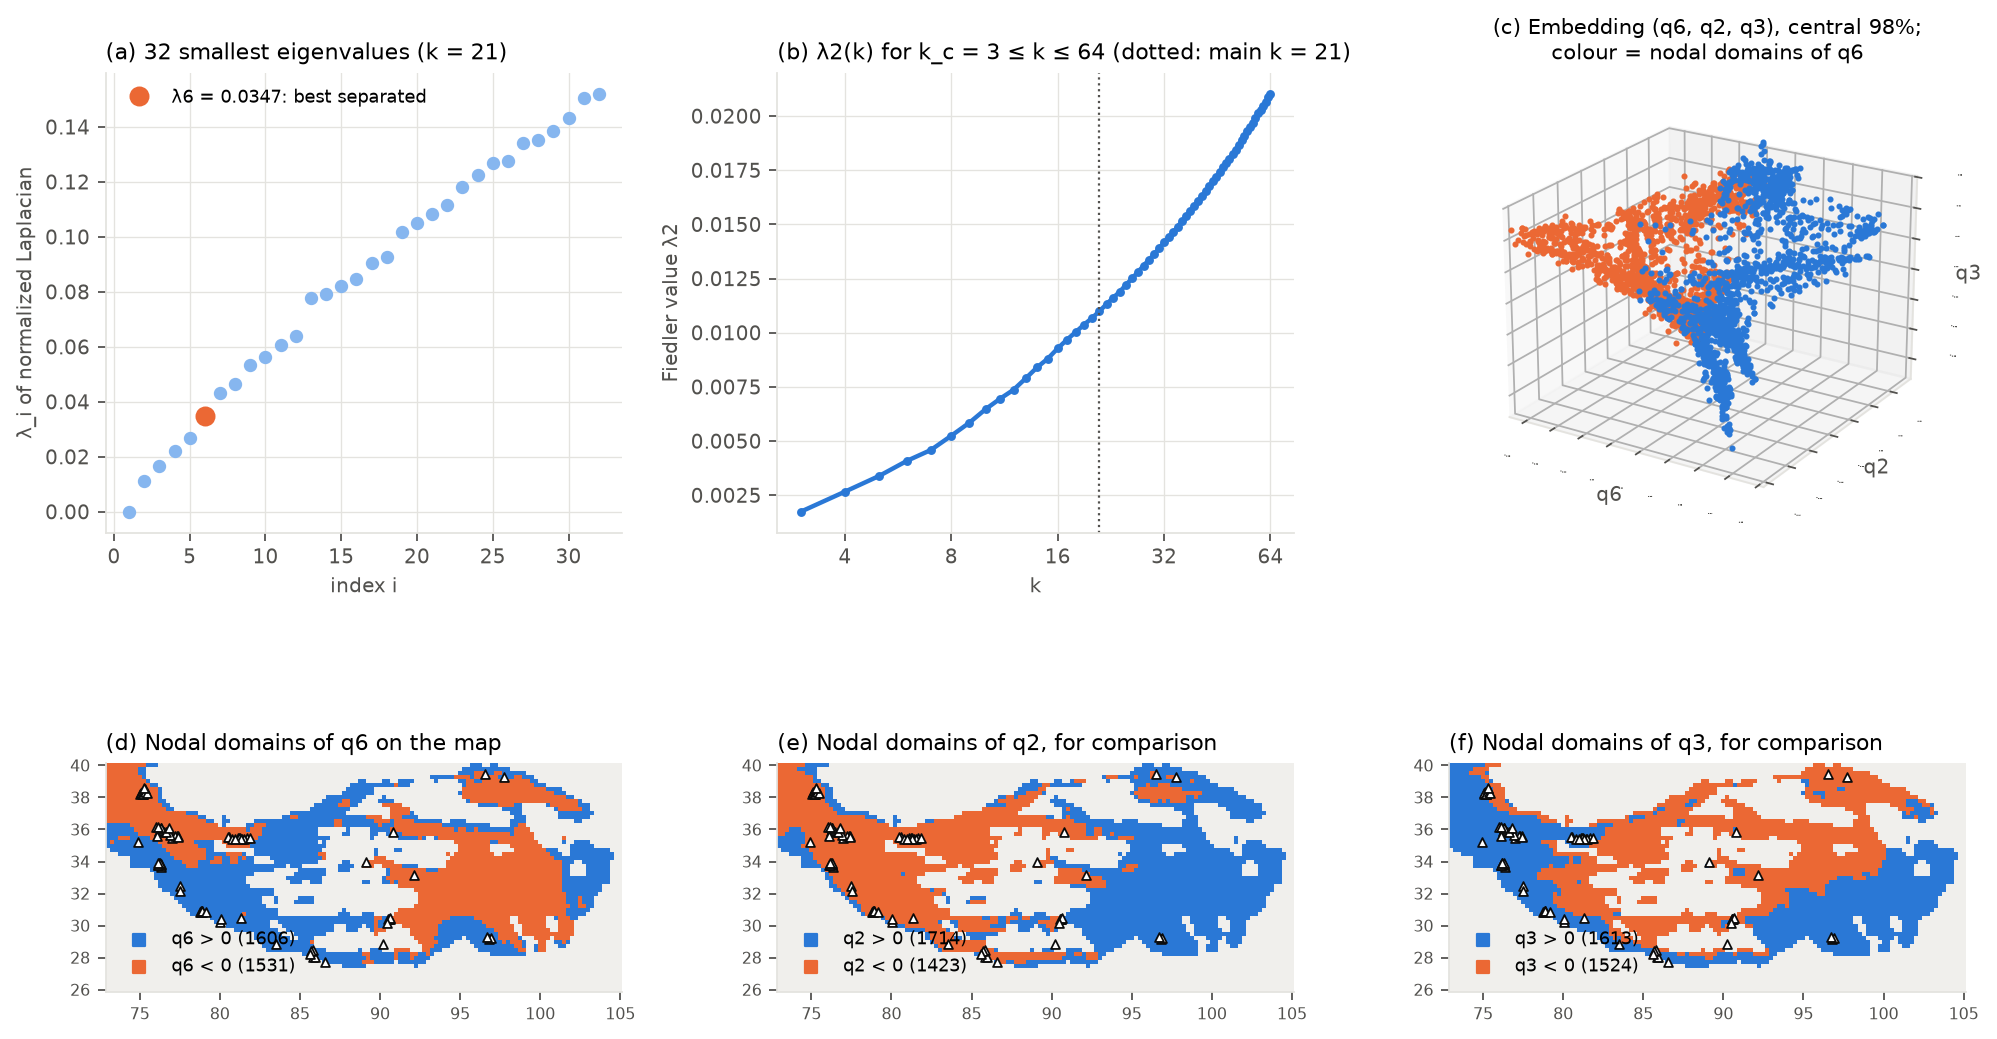
\includegraphics[width=\textwidth]{e5_spectrum.png}
  \caption{(a) The 32 smallest eigenvalues of $\hat L$ ($k=21$); orange: the
  best-separated one. (b) $\lambda_2$ versus $k$ for $3 \le k \le 64$. (c) Vertices in
  $(q_6,q_2,q_3)$, coloured by the nodal domains of $q_6$ (axes clipped to the central
  98\%). (d) Nodal domains of $q_6$ on the map. (e, f) Nodal domains of $q_2$ and $q_3$,
  for comparison.}
  \label{fig:e5}
\end{figure}

%=======================================================================
\section*{E-6 \quad Other methods: clustering, a spatial graph, year-by-year graphs}

\textbf{Spectral clustering} (Ng--Jordan--Weiss \cite{ng2002}: rows of
$[q_1, q_2, q_3]$ normalised to unit length, then $k$-means) with $K = 3$ gives three
regions (Fig.~\ref{fig:e6}a,b; Table~\ref{tab:regions}). They match the glacier regions of
Yao et al.\ almost perfectly: regions V (41/41) and IV (19/20) fall in the \emph{west};
II (5/5), VI (3/3) and VII (2/2) in the \emph{interior}; I (3/3) in the \emph{southeast}.
That is 73 of the 74 glaciers outside the mixed central Himalaya (region III, split 3/1/4).
This is the westerly / transition / monsoon pattern, recovered without any precipitation
data (H1).

\begin{table}[h]
\centering\small
\resizebox{\textwidth}{!}{%
\begin{tabular}{lrcccccc}
\toprule
Region & vertices & mean position & elevation & snow days & season$^*$ & peak & glacier regions \\
\midrule
West      & 721  & $79.1^\circ$E, $34.5^\circ$N & 4,731\,m & 266 & 16 Oct -- 21 Jun & 7.3\,cm, 2 Feb & V, IV \\
Interior  & 1,316 & $89.6^\circ$E, $34.5^\circ$N & 4,600\,m & 136 & 26 Oct -- 18 Apr & 3.0\,cm, 30 Nov & II, VI, VII \\
Southeast & 1,100 & $95.8^\circ$E, $32.3^\circ$N & 4,150\,m & 142 & 13 Nov -- 22 Apr & 6.0\,cm, 8 Jan & I \\
\bottomrule
\end{tabular}}
\caption{The three regions. $^*$Median dates on which a cell's mean depth first rises
above, and last falls below, 30\% of its maximum.}
\label{tab:regions}
\end{table}

\textbf{A spatial graph as a check.} The features contain no location. We therefore build
a second graph on the same vertices, with an edge between map neighbours (8-neighbours,
i.e.\ an rNN graph with $r$ = one cell):
\begin{itemize}\setlength\itemsep{0.1em}
  \item \emph{Contiguity.} 88.2\% of map-neighbour pairs are in the same region, against
        35.1\% after shuffling the labels. The regions are spatially coherent.
  \item \emph{Boundaries.} The feature distance between map neighbours has median 0.13
        inside a region and 0.21 across a border. The 10\% largest jumps lie on region
        borders 53\% of the time, although only 11.8\% of map edges are border edges. The
        sharpest jumps run along the outer rim of the plateau (Fig.~\ref{fig:e6}c).
  \item \emph{Long edges.} 6.2\% of kNN edges join cells more than 1,000\,km apart, and
        90\% of these stay inside one region: the graph links distant places with similar
        snow seasons, not just nearby ones.
\end{itemize}

\textbf{Louvain} modularity clustering \cite{blondel2008} on the weighted kNN graph gives
15 communities. Their purity with respect to the three spectral regions is 0.91, so
Louvain subdivides the regions rather than cutting across them.

\textbf{Year-by-year graphs (H2).} We built one graph per snow year (that year's features,
$k=21$, $K=3$, labels matched to the 14-year partition). Each year agrees with the
14-year partition on 57--87\% of vertices. 38\% of vertices keep their region in at least
12 of the 14 years (\emph{core}), and 19\% keep it in at most 7 (\emph{transition}). The
core is concentrated in the west: 54\% of west vertices are core, against 41\% of
interior and 25\% of southeast vertices (Fig.~\ref{fig:e6}d). For each border we measure
its sharpness (gradient of the $(q_2,q_3,q_4)$ embedding painted on the map) and its
stability:

\begin{center}\small
\begin{tabular}{lrccc}
\toprule
Cells & $n$ & embedding gradient & switching ($\le 7/14$ years) & clustering coeff.\\
\midrule
not on a border      & 2116 & 0.25 & 16\% & 0.48 \\
west $|$ interior    & 521  & 0.75 & 14\% & 0.41 \\
west $|$ southeast   & 219  & 0.61 & 24\% & 0.50 \\
interior $|$ southeast & 358 & 0.38 & 44\% & 0.43 \\
\bottomrule
\end{tabular}
\end{center}

The west--interior border is a \textbf{sharp, stable divide}: its gradient is 3.0$\times$
that of non-border cells, and its cells switch regime no more often than non-border cells.
The interior--southeast border is a \textbf{gradual, shifting belt}: its gradient is only
1.5$\times$, and 44\% of its cells switch. The west--southeast border is the narrow strip
along the western and southern Himalayan rim, and lies in between.

\textbf{Sensor check (H3).} The SSM/I $\to$ SSMIS change happens in snow year 2008/09.
Before it, no vertex is ever snow-free for a whole year; from 2008/09 on, 0--9 are
(mean 4.5). The per-year $\lambda_2$ also drops from a mean of 0.0170 to 0.0142. Two
independent statistics step at the same year, which points to an instrument effect
(Fig.~\ref{fig:e6}e). The E-1 comparison agrees: for every feature, graphs from the two
eras share fewer neighbours than graphs from random halves of the years.

\begin{figure}[h]
  \centering
  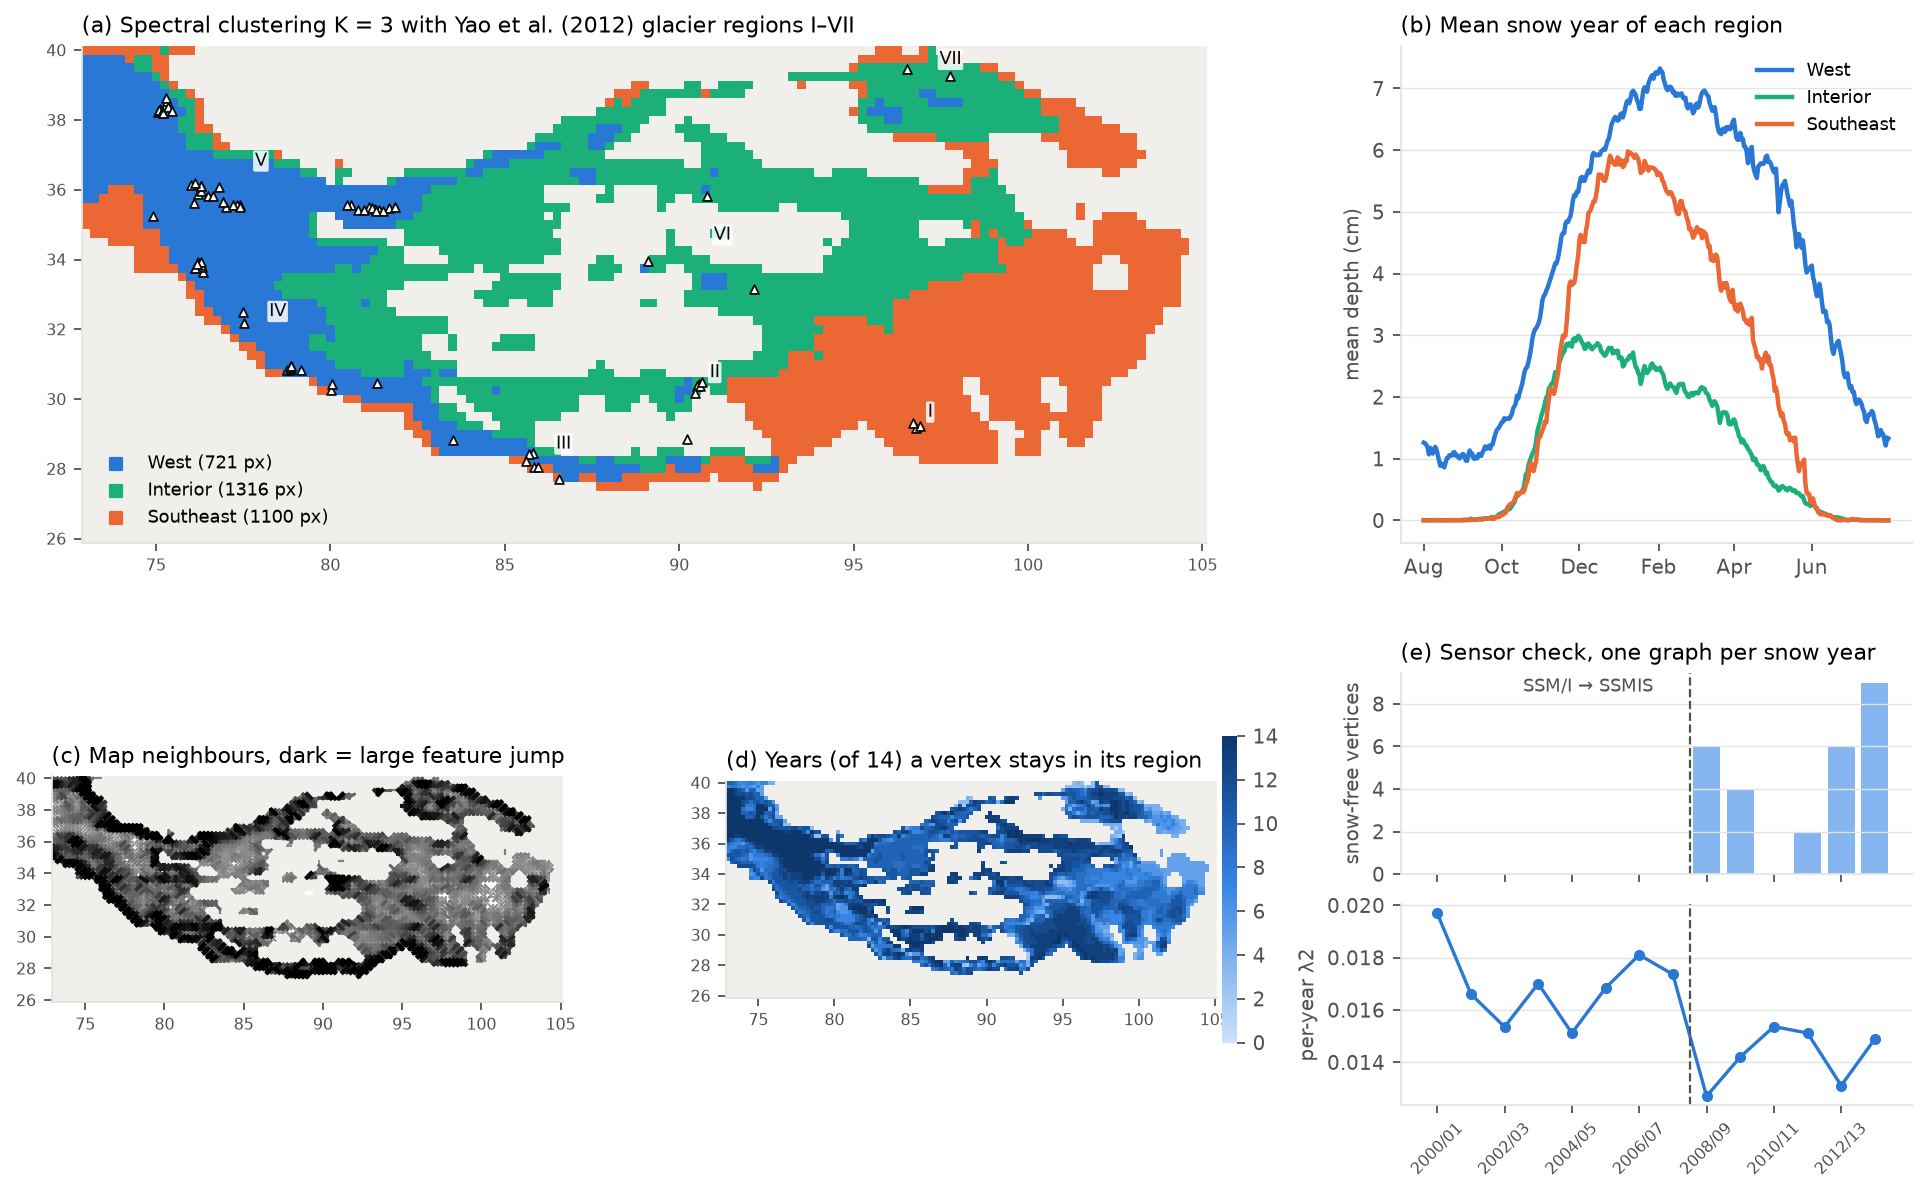
\includegraphics[width=\textwidth]{e6_regions.png}
  \caption{(a) Spectral clustering with $K=3$ and the glacier regions of Yao et al.
  (b) Mean snow year of each region. (c) Map-neighbour pairs; darker = larger feature
  distance. (d) Number of the 14 snow years in which a vertex is in its 14-year region.
  (e) Snow-free vertices and $\lambda_2$ of the per-year graphs; dashed: the sensor
  change.}
  \label{fig:e6}
\end{figure}

%=======================================================================
\clearpage
\section*{E-7 \quad Discussion}

\textbf{Key findings.}
\begin{enumerate}\setlength\itemsep{0.15em}
  \item \textbf{Snow alone recovers the climate regions (H1).} The graph separates a
        persistent-snow west, a thin-snow interior and a deep-seasonal southeast. They are
        spatially coherent, match the westerly / transition / monsoon glacier regions of
        Yao et al.\ (73 of 74 glaciers), and are not explained by elevation. The result
        is robust to $k$ (8--64), the time cells, the snow-day threshold and the metric.
  \item \textbf{The time scale of the gradient matters.} The climate signal sits in
        changes over weeks to months; day-to-day changes are dominated by retrieval
        flicker. A multi-scale gradient is the most reliable of the 13 features tested.
        Features that keep the amount of snow follow elevation instead.
  \item \textbf{The boundaries are of two kinds (H2).} The westerly region is bounded by a
        sharp, stable divide. The interior and the southeast are separated by a broad belt
        that shifts from year to year. The graph never splits into regions for any
        $k \ge 3$, the spectrum has no strongly isolated eigenvalue, and the embedding is
        one connected body with arms. Snow seasons therefore vary continuously, with one
        steep step at the edge of the westerly region.
  \item \textbf{The snow-season space is low-dimensional.} A clustering coefficient between
        those of 3-D and 4-D random points suggests three or four underlying parameters.
        Natural candidates are the start and end of the season and the speeds of
        accumulation and melt.
\end{enumerate}

\textbf{Confounds and limitations (H3).}
(i) \emph{Glacier ice.} The west keeps about 1.1\,cm of ``snow'' through August, probably
glacier ice seen by the radiometer, so the west region may partly reflect glacier cover.
The HOG ignores a constant offset, but the summer signal is not perfectly constant. Next
step: use the glacier fraction of each cell (Second Glacier Inventory of China) as a
covariate.
(ii) \emph{Sensor changes.} The step at 2008/09 means that year-to-year differences
(including border shifts) are partly instrumental. Next step: extend to 1979--2020 and
check every sensor change.
(iii) \emph{The number of regions.} $K = 3$ was imposed; the spectrum does not single out
three clusters. The three regions are supported by the external checks, not by an
eigengap.
(iv) \emph{Resolution.} The $\sim$25\,km microwave footprint blurs narrow ranges, which is
why the central Himalaya (region III) is split. Names follow snow behaviour, not
climate: the ``southeast'' region also covers a strip along the Himalayan rim.

\textbf{Next steps for the project.} Add the glacier-fraction covariate; use all years to
separate climate from sensor; and move to the 3\,km multi-variable TPDC snow product
(snowmelt, rain-on-snow) to ask whether the regions also differ in \emph{how} snow melts.

%=======================================================================
\section*{Acknowledgements and references}

The datasets are provided by the National Tibetan Plateau / Third Pole Environment Data
Center (\url{https://data.tpdc.ac.cn}) under CC BY-NC-SA 4.0. Computation used Python
with NumPy, Matplotlib and NetworkX.
% TODO (authors): add any acknowledgement required by the course policy on collaboration and AI tools.

\renewcommand{\refname}{}
\vspace{-2.5em}
\begin{thebibliography}{99}\small\setlength\itemsep{0.1em}
\bibitem{che_data} Che, T., Dai, L., \& Li, X. (2015). Long-term series of daily snow depth dataset in China (1979--2025). National Tibetan Plateau Data Center. \url{https://doi.org/10.11888/Geogra.tpdc.270194}
\bibitem{che2008} Che, T., Li, X., Jin, R., Armstrong, R., \& Zhang, T. (2008). Snow depth derived from passive microwave remote-sensing data in China. \emph{Annals of Glaciology}, 49, 145--154.
\bibitem{dai2015} Dai, L., Che, T., \& Ding, Y. (2015). Inter-calibrating SMMR, SSM/I and SSMI/S data to improve the consistency of snow-depth products in China. \emph{Remote Sensing}, 7(6), 7212--7230.
\bibitem{dai2017} Dai, L., Che, T., Ding, Y., \& Hao, X. (2017). Evaluation of snow cover and snow depth on the Qinghai--Tibetan Plateau derived from passive microwave remote sensing. \emph{The Cryosphere}, 11(4), 1933--1948.
\bibitem{xiong_data} Xiong, C., Shi, J., Yao, R., Lei, Y., \& Pan, J. (2020). Snowmelt onset time of High Mountain Asia (1979--2018). National Tibetan Plateau Data Center. \url{https://doi.org/10.11888/Snow.tpdc.270307}
\bibitem{xiong2017} Xiong, C., Shi, J., Cui, Y., \& Peng, B. (2017). Snowmelt pattern over High-Mountain Asia detected from active and passive microwave remote sensing. \emph{IEEE Geoscience and Remote Sensing Letters}, 14, 1096--1100.
\bibitem{xiong2019} Xiong, C., Yao, R., Shi, J., Lei, Y., \& Pan, J. (2019). Changes in snow and ice melt timing over High Mountain Asia. \emph{Chinese Science Bulletin}, 64(27), 2885--2893 (in Chinese).
\bibitem{yao_data} Yao, T. (2019). Different glacier status with atmospheric circulations in Tibetan Plateau and surroundings (1970s--2000s). National Tibetan Plateau Data Center. \url{https://doi.org/10.11888/Glacio.tpdc.270100}
\bibitem{yao2012} Yao, T., Thompson, L., Yang, W., et al. (2012). Different glacier status with atmospheric circulations in Tibetan Plateau and surroundings. \emph{Nature Climate Change}, 2, 663--667.
\bibitem{dalal2005} Dalal, N., \& Triggs, B. (2005). Histograms of oriented gradients for human detection. \emph{CVPR 2005}, 886--893.
\bibitem{lindeberg1994} Lindeberg, T. (1994). \emph{Scale-Space Theory in Computer Vision}. Springer.
\bibitem{endres2003} Endres, D. M., \& Schindelin, J. E. (2003). A new metric for probability distributions. \emph{IEEE Transactions on Information Theory}, 49(7), 1858--1860.
\bibitem{radovanovic2010} Radovanovi\'c, M., Nanopoulos, A., \& Ivanovi\'c, M. (2010). Hubs in space: popular nearest neighbors in high-dimensional data. \emph{Journal of Machine Learning Research}, 11, 2487--2531.
\bibitem{zelnik2004} Zelnik-Manor, L., \& Perona, P. (2004). Self-tuning spectral clustering. \emph{Advances in Neural Information Processing Systems 17}.
\bibitem{ng2002} Ng, A. Y., Jordan, M. I., \& Weiss, Y. (2002). On spectral clustering: analysis and an algorithm. \emph{Advances in Neural Information Processing Systems 14}.
\bibitem{blondel2008} Blondel, V. D., Guillaume, J.-L., Lambiotte, R., \& Lefebvre, E. (2008). Fast unfolding of communities in large networks. \emph{Journal of Statistical Mechanics}, P10008.
\end{thebibliography}

\end{document}
